%%%%%%%%%%%%%%%%%%%%%%%%%%%%%%%%%%%%%%%%%%%%%%%%%%%%%%%%%%%%%%%%%%%%%%
% How to use writeLaTeX: 
%
% You edit the source code here on the left, and the preview on the
% right shows you the result within a few seconds.
%
% Bookmark this page and share the URL with your co-authors. They can
% edit at the same time!
%
% You can upload figures, bibliographies, custom classes and
% styles using the files menu.
%
%%%%%%%%%%%%%%%%%%%%%%%%%%%%%%%%%%%%%%%%%%%%%%%%%%%%%%%%%%%%%%%%%%%%%%

\documentclass[12pt]{article}

\usepackage{sbc-template}

\usepackage{graphicx,url}

%\usepackage[brazil]{babel}   
\usepackage[utf8]{inputenc}  

     
\sloppy

\title{Analise e testes a respeito do funcionamento de um SNIFFER }

\author{Esdras Fragoso da Silva Neto, Helbert Alves Monteiro da Silva }


\address{Universidade Federal do Piauí 
  (UFPI)\\ Campos Senador Helvídio Nunes de Barros \\ 
  Bacharelado em Sistemas de Informação \\  
  RUA Cícero Eduardo -- CEP 64600-000 -- Picos -- PI -- Brasil 
  \email{\{esdrasfragoso,helbert.monteiro0\}@gmail.com}
}

\begin{document} 

\maketitle

\begin{abstract}
  With the rapid growth of the use of computer networks, occasions of congestion, losses of packages, and constant attacks, this way it became necessary: a management, maintenance and monitoring of the network, to maintain it: mitigated, relieving the stress of the same , allowing packets to travel with minimal loss and improving the efficiency of device usage, with good management, commensurate with a resource saving the network can increase its capacity and supports an excessive load of users. For this reason the sniffer is used. Being decisive without network monitoring to troubleshoot and registrar
activities. various site sniffers are available in the market. This article discusses a Wireshark feature that is most commonly used and recommended sniffers. To illustrate all the features in an available tool, in addition to describing the efficiency in detecting malicious packets on any network, it has been tested through real-time network experience. Inferences performed without testing clearly describe how Wireshark capabilities
highlighting it as a strong intruder detector. It is important to
Wireshark as a network protocol analyzer and also
accentuates its flexibility as an open source and
to developers, in addition to features. All tests and procedures in the tool analysis process were done by capturing packages issued by a login application and password.
  
\end{abstract}
     
\begin{resumo} 
  Com crescimento vertiginoso do uso de redes de computadores, ocasionou congestionamentos, perdas de pacotes, além de ataques constantes. Desta forma, tornou-se necessário: a gestão, manutenção e o monitoramento da rede,  para mantê-la: suavisada, aliviando o estresse da mesma, permitindo que pacotes trafeguem com o mínimo de perdas possível e melhorando a eficiência do uso dos dispositivos, pois com um bom gerenciamento, cominando com uma economia de recursos, a rede pode aumentar sua capacidade e suportar a carga excessiva de usuários. Por esta razão o sniffer é usado. Sendo decisivo no monitoramento da rede para solucionar problemas e registrar
atividades de rede. Vários sniffers de pacotes estão disponíveis no mercado.  Este artigo aborda a funcionalidade do Wireshark que é o mais usado e recomendado sniffers. Para ilustrar todos os recursos que a ferramenta dispõe, além de descrever a eficiência na detecção de pacotes maliciosos em qualquer rede foi realizados testes através da experimentação em uma rede em tempo real. Inferências realizadas no teste descrevem claramente as capacidades do Wireshark
destacando-o como um forte detector de intrusão. É mister destacar o
trabalho da Wireshark como um analisador de protocolo de rede e também
acentua a sua flexibilidade como um utilitário de código aberto para permitir
aos desenvolvedores  adicionar possíveis funcionalidades.  Todos os testes e procedimentos no processo de análise da ferramenta foram feitos capturando pacotes emitidos por um aplicativo de login e senha.
\end{resumo}


\section{Introdução}

	Os últimos anos, testemunharam um grande aumento no uso de dispositivos móveis. provocando um aumento exponencial no uso de redes de computadores. Assim, pesquisas na área é de primordial importância para o melhoramento da qualidade de serviços da rede.

Um dos serviços vitaais ao funcionamento da rede é a segurança. Ligado ou não, entrada improvável e indesejada de usuários mal-intencionados e / ou pacotes de dados são uma grande preocupação. Os pacotes de dados são entidades básicas de todos os sistemas de comunicação. Portanto a segurança de uma rede implica, na dos pacotes de dados, pois se trata do bloco mais básico de comunicação envolvendo um fluxo de infinitas outras réplicas para transmitir informações
de um dispositivo para outro.

A identidade de qualquer pacote proveniente de qualquer fonte não confiável pode ser detectado estudando seus conteúdos. Este estudo de detecção e
apenas visualizando o conteúdo de um segmento de dados e seu pacote é
denominado como sniffing  ou  na nossa lingua cheiro de pacotes e quando um registro dessa informação é
preparado, a técnica é chamada de log de pacotes. Um pacote analisador é um software de computador ou hardware que pode interceptar
o tráfego de log que passa por uma rede digital ou parte de uma
rede. À medida que os fluxos de dados fluem através da rede, o sniffer
captura cada pacote e, eventualmente, decodifica e analisa o seu
conteúdo de acordo com a especificação apropriada.

Este artigo analisa o processo de cheirar pacotes por meio da ferramenta Wireshark que é uma rede de código aberto comumente disponível
analisador de protocolo, além de analisar as funcionalidades do mesmo, que são
muito convenientes para detectar qualquer entrada de pacote suspeito de qualquer fonte não confiável. Neste trabalho realizamos testes para observarmos o comportamento do Wireshark diante de algumas situações, os testes de captura de pacotes pela ferramenta Wireshark capturou pacotes de um aplicativo de login e senha que desenvolvemos para os testes.  

\section{Sniffers}
Um sniffer não é impreterivelmente malicioso. Deveras, esse tipo de ferramenta  é  frequentemente utilizado para monitorar e analisar o tráfego de rede, para detectar problemas e manter as coisas fluindo energeticamente. Todavia um Sniffers pode também ser utlizado com intenções maliciosas. 

Um Sniffers rastreia tudo o que passa por eles, incluindo senhas não criptografadas que hackers podem acessar e visualizar todas as contas que a atravessam a ferramenta. Além disso, um sniffer pode ser instalado em qualquer computador conectado a uma rede local sem precisar ser instalado no próprio dispositivo, em outras palavras, ele pode fascilmente não ser notado durante a conexão. 

Os Sniffers podem serem usados para defraudar dados, observar o fluxo de pacotes na rede e colher informações sobre os clientes da rede. comumente, o propósito final é a abdução de senhas e informações de contas bancárias e de sites de compras. 

Embora os sniffers não outorgados são potencialmente impossíveis de se perceber e podendo ser introduzidos teóricamente em  qualquer lugar, o que os torna profundamente perigosos para a segurança de uma rede. É presumível que um cliente comum da rede nunca venha a saber que um sniffer o espiona pela sua própia rede. Hipoteticamente, pode-se ter seu próprio sniffer e monitorar o fluxo de DNS para achar outros, mas para o usuário comum o que é mais  viável é dispor  de uma ferramenta antisniffer para detectar um agressor ou utilizar um software que oculte a navegação na internet.

\subsection{Como remover um sniffer}
Um dos métodos mais é utilizar um antivírus enérgico para localizar e excluir qualquer malware vinculado a um sniffer que possa ter sido executado. Porém, para excluir integralmente um sniffer de qualquer computador, torna-se necessario eliminar os documentos e as pastas vinguladas a ele. todavia, para retirar um sniffer que tenha sido executado ilícitamente na rede, é aconselhável utilizar um aplicativo ou ferramenta de segurança que disponha de um scanner de rede que a examinara a procura de distúrbios e o instruíra sobre como solucioná-los. 

\subsection{Evitar os Efeitos de um Sniffer}
A preferível modo de salvaguardar-se dos sniffers é criptografar todos os dados importantes ou seja dodos confidenciais, secretos, reservados ou íntimos transmitidos on-line. O antivírus pode ser de grande ajuda como instrumento secundário para salvaguarda-se dos efeitos de  sniffer, mas nada substituir a criptografia.

\section{WIRESHARK} \label{sec:firstpage}

Wireshark é o protocolo analisador de rede mais popular do mundo. Tem um conjunto de recursos, além de funcionar com a maioria das 
plataformas de computação, incluindo Windows, OS X, Linux e
UNIX. 
Profissionais de rede, especialistas em segurança, desenvolvedores e
Educadores de todo o mundo usam o Wireshark regularmente. O mesmo se encontra disponível gratuitamente
com fonte aberta. Foi desenvolvido e mantido por uma
equipe global de especialistas em protocolo, tornando-se um exemplo de
tecnologia disruptiva. 

O Wireshark é uma aplicação de computador com sniffer de pacotes grátis.
É usado para solução de problemas, análises, softwares e
desenvolvimento de protocolos de comunicação e educação. O mesmo possui ferramentas para capturar, visualizar e analisar pacotes de dados. Além disso, possui um sofisticado protocolo para redes sem fio,
fornecendo suporte e análise, que ajudam administradores a solucionar problemas de conexão em redes sem fio. 

Com o suporte apropriado do driver, o Wireshark pode
capturar o tráfego "do ar" e decodificá-lo em um formato que
ajuda os administradores a rastrear o que está causando problemas
de: desempenho, conectividade intermitente e outros comuns
problemas.

O Wireshark fornece aos usuários a capacidade de capturar
pacotes que viajam por toda a rede em uma determinada
interface e em um momento específico. Uma das principais ferramentas é a
ferramenta de captura. O menu "Capturar" é fornecido para que os usuários possam
executar capturas de pacote, além de ter disponível várias opções
para adequar as situações e as condições que os analistas
tem na mente enquanto executa o processo de captura dos pacotes. É possível ainda definir filtros para evitar capturar tráfego indesejado

Embora o  wireshark possua uma vasta quantidade de recursos, ele  tem algumas limitações justamente por não ser um
sistema de detecção de intrusão. Não avisará quando
alguém fizer coisas estranhas na  rede, além de que também não manipulará coisas
na rede, por outro lado, o Wireshark tem uma GUI amigável para os usuários.  

\section{Análise de tráfico na rede}

A análise do tráfego de rede pode ser definida como: "a inferência das informações obtidas com a observação do fluxo de dados na rede ". Análise em geral é, portanto, análise do tráfego da rede, que pode ser categorizada em: análise em tempo real, análise em bote e análise forense.
\subsection{Análise em Tempo Real}
A análise em tempo real:  É realizada ao longo dos dados, pois é obtida, usando pequenos lotes, muitas vezes chamados de buffers para analise eficientemente os dados. O tempo de resposta deste tipo de análise é entendida como o tempo decorrido entre um certo evento que ocorre e é computado ou detectado, é baixo graças ao na baixa taxa atraso na obtenção de dados e ao fato de que em tempo real as análises são totalmente automatizadas. Análise em tempo real, porém, geralmente possui requisitos e recursos computacionais elevados.

\subsection{Análise de Batched}
A análise de Batched realiza análises periodicamente, onde o período é suficiente para acumular dados nos chamados lotes de dados. Dependendo das políticas de lotes, tempo de resposta e recursos computacionais associados os requisitos podem ser maiores ou inferiores, mas, em geral, eles oferecem um maior tempo de resposta e menor computação de requisitos e recursos do que a análise em tempo real (embora requerem um tamanho de armazenamento maior).
\subsection{Análise Forense}
A análise forense é análise realizado quando ocorre um evento específico (análise desencadeada). Um exemplo típico de análise forense é a análise realizada quando uma intrusão é detectada em um host particular. Este tipo de análise exige que os dados tenham sido anteriormente armazenados para ser analisado, e também pode exigir o uso de intervenção humanos. 

\section{Experimento com o Wireshark}

	Para demonstrar melhor como um sniffer funciona na prática, utilizamos neste trabalho o Wireshark para monitorar uma rede. O uso do Wireshark foi mais especificamente usado para capturar dados desprotegidos que trafegam pela rede e para isso nós criamos uma aplicação mobile bem simples, que funciona no modo cliente-servidor online, conectados por um Web-Service. A aplicação foi desenvolvida para a plataforma Android e faz apenas cadastros e autenticação de usuários, porém, sem a segurança necessária para que os dados possam trafegar de forma segura na rede entre o cliente e o servidor.

	Não iremos detalhar muito sobre como foi feito o aplicativo e como foi implementado o servidor, pois o objetivo deste tópico é demonstrar a captura dos dados na rede através do Wireshark.
    
	A simulação aconteceu entre dois dispositivos móveis com o aplicativo devidamente instalado e o servidor. Primeiro iniciamos o monitoramento de todo o tráfego da rede, como é mostrado na figura~\ref{fig:exampleFig1}. 

\begin{figure}[ht]
\centering
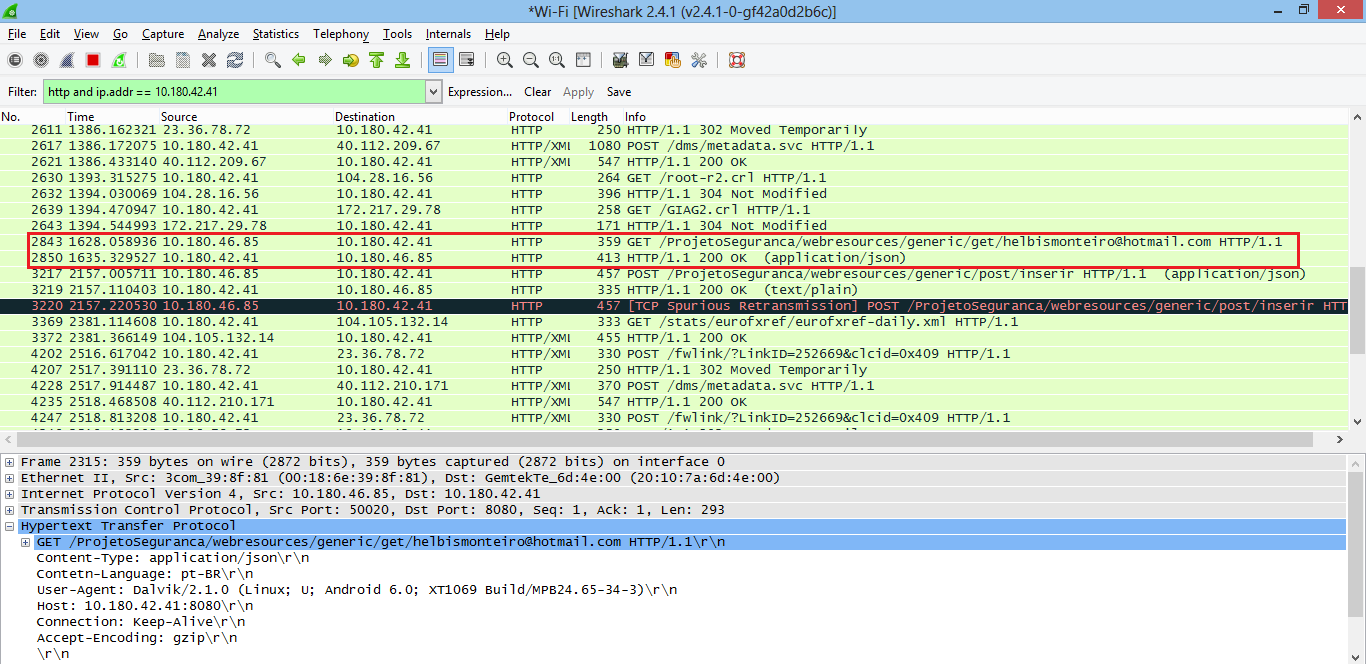
\includegraphics[width=.5\textwidth]{01.png}
\caption{Wireshark}
\label{fig:exampleFig1}
\end{figure}

Após iniciar a captura dos dados, fizemos um filtro para encontrar mais facilmente o tráfego de dados com o servidor. Para isso, filtramos pelo método Http e pelo Ip de origem e destino do servidor, para pegar as requisições e respostas com os clientes. Observe na figura ~\ref{fig:exampleFig2} em destaque de vermelho o filtro usado.

\begin{figure}[ht]
\centering
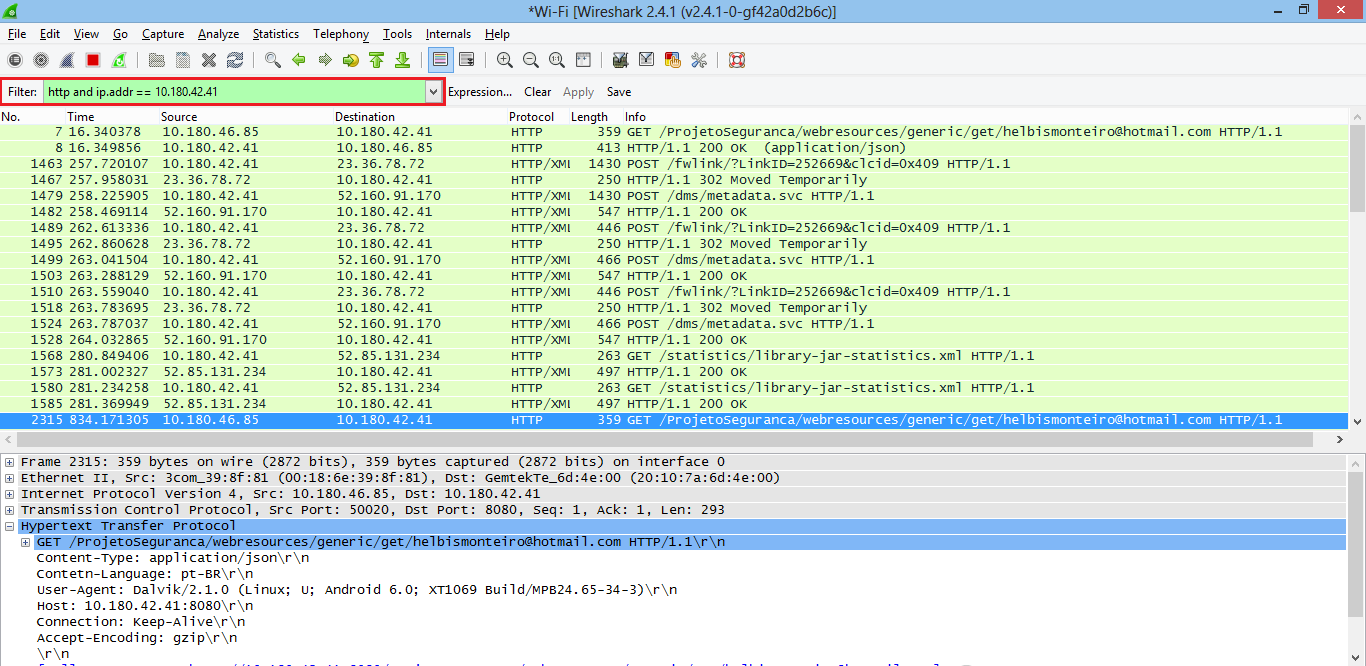
\includegraphics[width=.5\textwidth]{filtro.png}
\caption{Filtro}
\label{fig:exampleFig2}
\end{figure}

Com o filtro, podemos encontrar mais facilmente as requisições enviadas pelo cliente e a resposta do servidor e dessa forma capturar os dados dos pacotes. Observe em destaque de vermelho nas próximas imagens (figuaras 3 e 4) o tráfego entre o servidor e o primeiro dispositivo e os dados capturados nos pacotes respectivamente.  

\begin{figure}[ht]
\centering
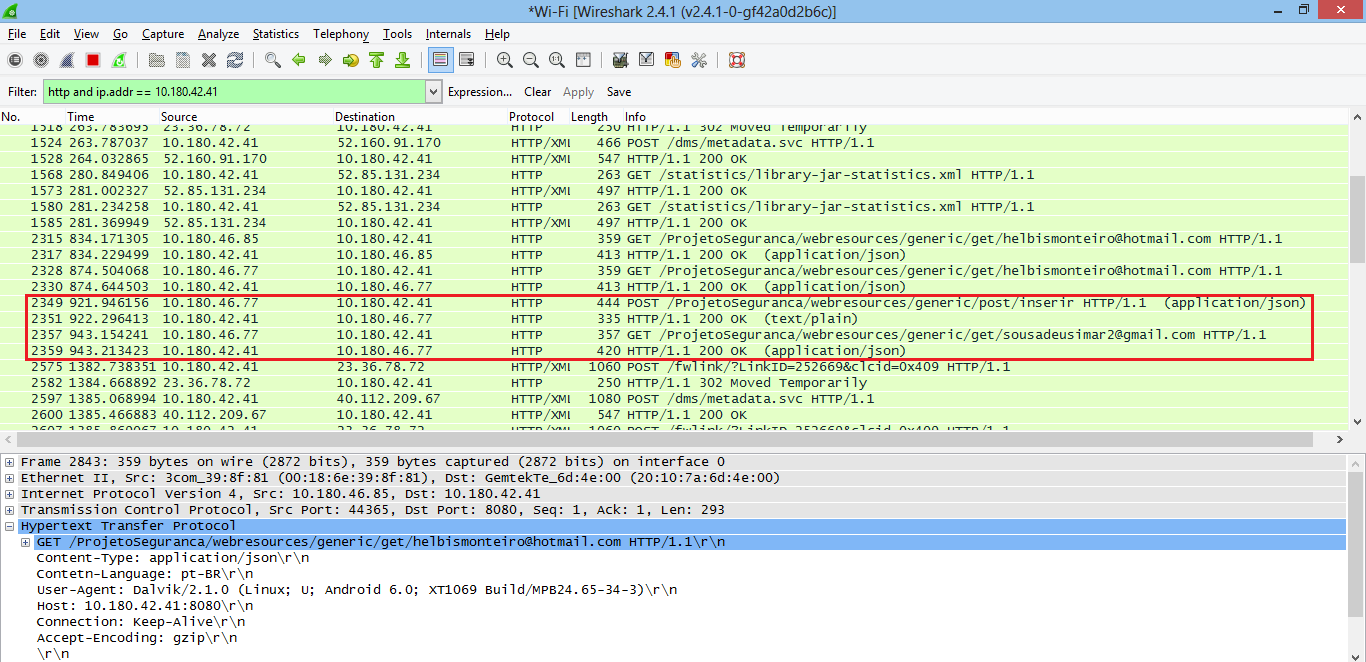
\includegraphics[width=.5\textwidth]{encontrar.png}
\caption{Filtro}
\label{fig:exampleFig3}
\end{figure}

\begin{figure}[ht]
\centering
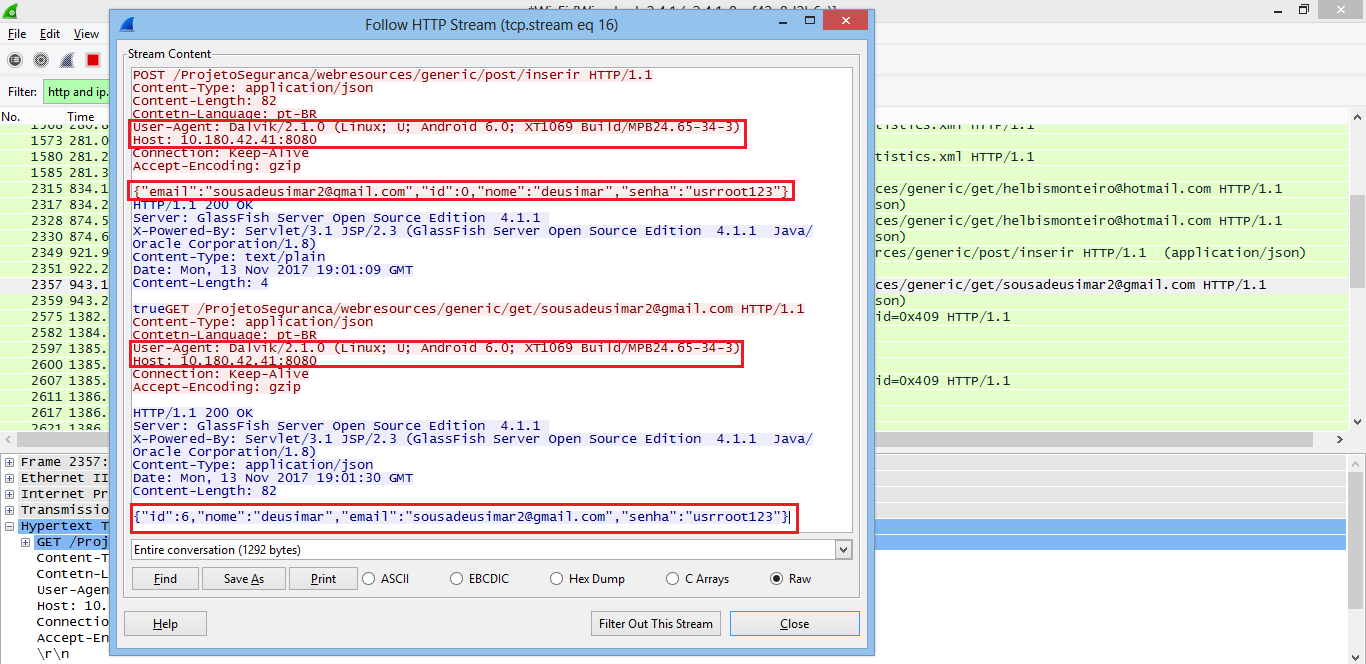
\includegraphics[width=.5\textwidth]{3.png}
\caption{Filtro}
\label{fig:exampleFig4}
\end{figure}

Nas figuras~\ref{fig:exampleFig5} e ~\ref{fig:exampleFig6} que estão destacadas de vermelho é possível ver também o tráfego e a captura dos dados do segundo dispositivo respectivamente.

\begin{figure}[ht]
\centering
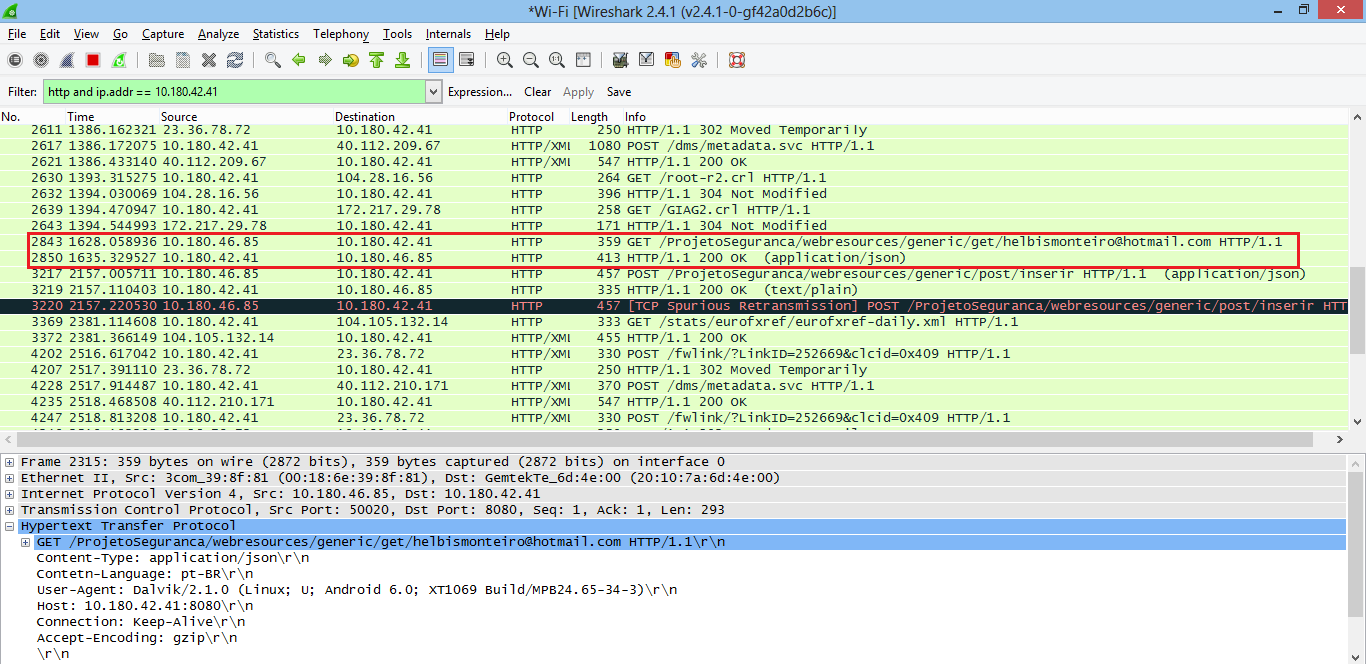
\includegraphics[width=.5\textwidth]{01.png}
\caption{Filtro}
\label{fig:exampleFig5}
\end{figure}

\begin{figure}[ht]
\centering
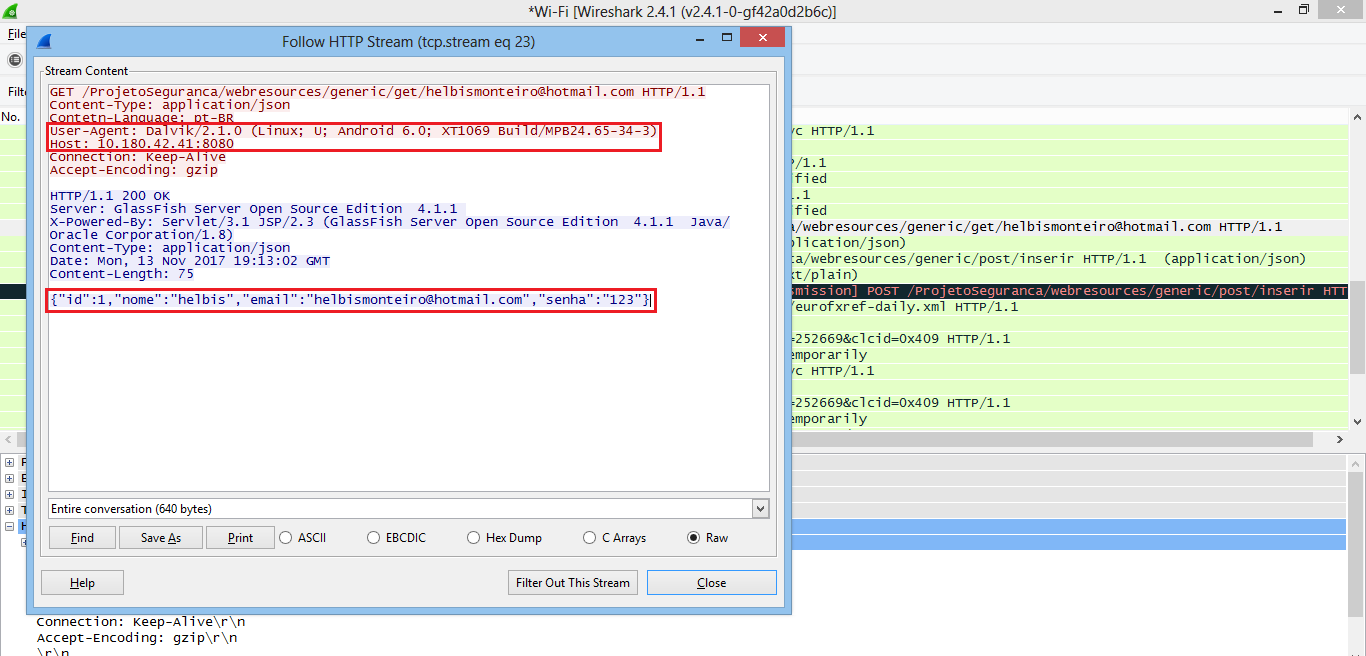
\includegraphics[width=.5\textwidth]{02.png}
\caption{Filtro}
\label{fig:exampleFig6}
\end{figure}


\subsection{Conclusão}

	Com os estudos abordados e os testes realizados neste trabalho, observamos a eficiência da ferramenta Wireshark, tanto para o uso da segurança de uma rede detectando falhas e intrusões através do monitoramento dos dados, como também para espionagem, capturando dados para serem decodificados a fim de obter informações privilegiadas. 

Compreendemos nos testes que a falta da implementação de segurança nas aplicações que usam uma rede para trafegar dados, pode comprometer um dos pilares da segurança da informação, que é a confidencialidade, a qual significa garantir que as informações não serão conhecidas por pessoas que não estejam autorizadas a elas. Por isso, é importante o uso de uma criptografia forte dos dados quando sigilosos antes de enviá-los pela rede, para tentar garantir, que mesmo que interceptados, não sejam decifrados pelo espião. Este é apenas um exemplo de tantos outros que buscam garantir a segurança da informação nas redes de computador, 

Conclusão do teste foi que o Wireshark é uma ótima ferramenta para auxiliar na implementação de uma rede segura.

\bibliographystyle{sbc}
\bibliography{sbc-template}

\end{document}
